 
\begin{figure}[H]
 \centering
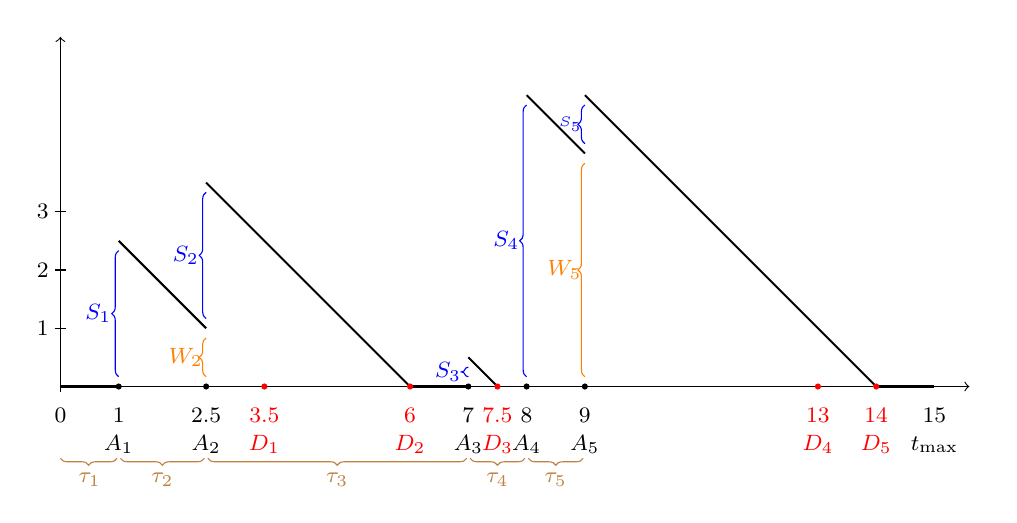
\begin{tikzpicture}[scale=0.74]
%\draw[help lines, color=gray!30, dashed] (-4.9,-4.9) grid (4.9,4.9);


 \draw[->] (0,0)--(15.6,0) node[right]{};
 \draw[->] (0,0)--(0,6) node[right]{};
 \draw (0,-0.1)--(0,0.1) node[above]{};
 \node () at (0.0,-0.5) {\footnotesize{$0$}};
 \node (n0) at (0.0,0.3) {};
 
 \draw[-] (-0.1,1)--(0.1,1) node[left]{\footnotesize{1 \ }};
 \draw[-] (-0.1,2)--(0.1,2) node[left]{\footnotesize{2 \ }};
 \draw[-] (-0.1,3)--(0.1,3) node[left]{\footnotesize{3 \ }};





\node[color=red]  at (3.5,-1.0) {\footnotesize{$D_1$}};
\node[color=red]  at (6.0,-1.0) {\footnotesize{$D_2$}};
\node[color=red]  at (7.5,-1.0) {\footnotesize{$D_3$}};
\node[color=red]  at (13,-1.0) {\footnotesize{$D_4$}};
\node[color=red]  at (14,-1.0) {\footnotesize{$D_5$}};



\node (a1) at (1,-0.5) {\footnotesize{$1$}};
\node (a1b) at (1,-1.0) {\footnotesize{$A_1$}};
\node (a2) at (2.5,-0.5) {\footnotesize{$2.5$}};
\node (a2b) at (2.5,-1.0) {\footnotesize{$A_2$}};
\node (a3) at (7,-0.5) {\footnotesize{$7$}};
\node (a3b) at (7,-1.0) {\footnotesize{$A_3$}};
\node (a4) at (8,-0.5) {\footnotesize{$8$}};
\node (a4b) at (8,-1.0) {\footnotesize{$A_4$}};
\node (a5) at (9,-0.5) {\footnotesize{$9$}};
\node (a5b) at (9,-1.0) {\footnotesize{$A_5$}};


\node[color=red]  (p35) at (3.5,-0.5) {\footnotesize{$3.5$}};
\node[color=red]  (p50) at (6.0,-0.5) {\footnotesize{$6$}};
\node[color=red]  (p75) at (7.5,-0.5) {\footnotesize{$7.5$}};
\node[color=red]  (p130) at (13.0,-0.5) {\footnotesize{$13$}};
\node[color=red]  (p140) at (14.0,-0.5) {\footnotesize{$14$}};
\node[color=black]  (ptmax) at (15.0,-0.5) {\footnotesize{$15$}};

\node[color=black]  (p100) at (15.0,-1.0) {\footnotesize{$t_{\rm max}$}};




\node (N1a) at (1,0) {};
\node (N1b) at (1,2.5) {};


%\fill (1,2.5)  circle[radius=1.5pt];

\node[color=blue] (s1) at (0.65,1.25) {\footnotesize{$S_1$}};
 \draw[decoration={brace }, decorate, color=blue] (N1a) -- (N1b) node {};


  %\draw [decorate, decoration={brace,amplitude=20pt,raise=2pt,mirror}] (N1a) -- (N1b)
   %         node [midway, xshift=3mm, yshift=-1mm,auto, swap, outer sep=10pt,font=\tiny]{};


\draw[line width=0.35mm] (0,0)--(1.0,0);
  \node (N2a) at (2.5,0) {};
\node (N2b) at (2.5,1) {};

\draw[line width=0.25mm] (1.0,2.5)--(2.5,1.);

\node[color=orange] (w2) at (2.15,0.5) {\footnotesize{$W_2$}};
 \draw[decoration={brace }, decorate, color=orange] (N2a) -- (N2b) node {};


\node (N3a) at (2.5,1) {};
\node (N3b) at (2.5,3.5) {};

\node[color=blue] (s1) at (2.15,2.25) {\footnotesize{$S_2$}};
 \draw[decoration={brace }, decorate, color=blue] (N3a) -- (N3b) node {};


 \draw[line width=0.25mm] (2.5,3.5)--(6.0,0);
 \draw[line width=0.35mm] (6,0)--(7.0,0);

 \node (N4a) at (7,0) {};
\node (N4b) at (7,0.5) {};

\node[color=blue] (s1) at (6.65,0.25) {\footnotesize{$S_3$}};
 \draw[decoration={brace }, decorate, color=blue] (N4a) -- (N4b) node {};

\draw[line width=0.25mm] (7,0.5)--(7.5,0);


 \node (N5a) at (8,0) {};
\node (N5b) at (8,5) {};

\node[color=blue] (s1) at (7.65,2.5) {\footnotesize{$S_4$}};
 \draw[decoration={brace }, decorate, color=blue] (N5a) -- (N5b) node {};

\draw[line width=0.25mm] (8,5)--(9,4);

 \node (N6a) at (9,0) {};
\node (N6b) at (9,4) {};

\node[color=orange] (w2) at (8.65,2) {\footnotesize{$W_5$}};
 \draw[decoration={brace }, decorate, color=orange] (N6a) -- (N6b) node {};

  \node (N7a) at (9,4) {};
\node (N7b) at (9,5) {};

\node[color=blue] (s1) at (8.75,4.5) {\tiny{$S_5$}};
 \draw[decoration={brace }, decorate, color=blue] (N7a) -- (N7b) node {};

 \draw[line width=0.25mm] (9,5)--(14,0);

 \draw[line width=0.35mm] (14,0)--(15,0);

%
%  \node (m1a) at (1.03,1.0) {};
% \node (m1b) at (3.47,1.0) {};
%
%
% \node[color=blue] (s1) at (2.25,1.5) {\footnotesize{$S_1$}};
%  \draw[decoration={brace }, decorate, color=blue] (m1a.north) -- (m1b.north) node {};
%
%
%
%  \node (m2a) at (2.53,2.0) {};
% \node (m2b) at (3.47,2.0) {};
%
%  \node[color=orange] (w2) at (3.0,2.5) {\footnotesize{$W_2$}};
%
%  \draw[decoration={brace }, decorate, color=orange] (m2a.north) -- (m2b.north) node  {};
%
%
%   \node[color=blue] (s2) at (4.75,1.5) {\footnotesize{$S_2$}};
%
%  \node (m25a) at (3.53,1.0) {};
% \node (m25b) at (5.97,1.0) {};
%
%  \draw[decoration={brace }, decorate, color=blue] (m25a.north) -- (m25b.north) node  {};
%
%  \node (m3a) at (7.03,1.0) {};
% \node (m3b) at (7.47,1.0) {};
%
%  \node[color=blue] (s3) at (7.25,1.5) {\footnotesize{$S_3$}};
%  \draw[decoration={brace }, decorate, color=blue] (m3a.north) -- (m3b.north) node  {};
%
%
%
%
%  \node (m4a) at (8.03,1.0) {};
% \node (m4b) at (12.97,1.0) {};
%
%  \node[color=blue] (s4) at (11,1.5) {\footnotesize{$S_4$}};
%  \draw[decoration={brace }, decorate, color=blue] (m4a.north) -- (m4b.north) node  {};
%
%
%
%
%
%  \node (m5a) at (9.03,2.0) {};
% \node (m5b) at (12.97,2.0) {};
%
%  \node[color=orange] (s5) at (11,2.5) {\footnotesize{$W_5$}};
%  \draw[decoration={brace }, decorate, color=orange] (m5a.north) -- (m5b.north) node  {};
%
%
%
%
%  \node (m6a) at (13.03,1.0) {};
% \node (m6b) at (13.97,1.0) {};
%  \node[color=blue] (s5) at (13.5,1.5) {\footnotesize{$S_5$}};
%  \draw[decoration={brace }, decorate, color=blue] (m6a.north) -- (m6b.north) node  {};

%
%  \draw[line width=0.5mm] (0.0,0)--(1.0,0);
%  \draw[line width=0.5mm] (1.0,1.0)--(2.5,1.0);
%
%  \draw[line width=0.5mm] (2.5,2.0)--(3.5,2.0);
%
%  \draw[line width=0.5mm] (3.5,1.0)--(6,1.0);
%
%  \draw[line width=0.5mm] (6.0,0.0)--(7.0,0.0);
%
%  \draw[line width=0.5mm] (7.0,1.0)--(7.5,1.0);
%
%
%  \draw[line width=0.5mm] (7.5,0)--(8,0);
%
%
%
%  \draw[line width=0.5mm] (8.0,1.0)--(9,1.0);
%
%
%  \draw[line width=0.5mm] (9.0,2.0)--(13,2.0);
%
%
%  \draw[line width=0.5mm] (13,1.0)--(14,1.0);
%  \draw[line width=0.5mm] (14,0.0)--(15.0,0.0);
%  \draw[line width=0.3mm] (15.0,-0.1)--(15.0,0.1);
%
%
 
 \node (tau0) at (0,-1.4) {};
\node (tau1L) at (0.97,-1.4) {};
\node (tau1R) at (1.03,-1.4) {};
\node (tau2L) at (2.47,-1.4) {};
\node (tau2R) at (2.53,-1.4) {};
\node (tau3L) at (6.97,-1.4) {};
\node (tau3R) at (7.03,-1.4) {};
\node (tau4L) at (7.97,-1.4) {};
\node (tau4R) at (8.03,-1.4) {};
\node (tau5L) at (8.97,-1.4) {};
\node (tau5R) at (9.03,-1.4) {};




 %\node[color=orange] (w2) at (3.0,2.5) {\footnotesize{$w_2$}};
 
 \draw[decoration={brace, mirror}, decorate, color=brown] (tau0.north) -- (tau1L.north) node  {};
 \draw[decoration={brace, mirror}, decorate, color=brown] (tau1R.north) -- (tau2L.north) node  {};
 \draw[decoration={brace, mirror}, decorate, color=brown] (tau2R.north) -- (tau3L.north) node  {};
 \draw[decoration={brace, mirror}, decorate, color=brown] (tau3R.north) -- (tau4L.north) node  {};
 \draw[decoration={brace, mirror}, decorate, color=brown] (tau4R.north) -- (tau5L.north) node  {};
\node[color=brown]  at (0.5,-1.6) {\footnotesize{$\tau_1$}};
\node[color=brown]  at (1.75,-1.6) {\footnotesize{$\tau_2$}};
\node[color=brown]  at (4.75,-1.6) {\footnotesize{$\tau_3$}};
\node[color=brown]  at (7.5,-1.6) {\footnotesize{$\tau_4$}};
\node[color=brown]  at (8.5,-1.6) {\footnotesize{$\tau_5$}};
 
 
 
 
 %\draw[line width=0.5mm, dashed] (14.5,0.0)--(14.95,0.0);
 
 \tikzset{cross/.style={cross out, draw=black, minimum size=2*(#1-\pgflinewidth), inner sep=0pt, outer sep=0pt},
%default radius will be 1pt. 
cross/.default={11pt}}

\tikzset{
    cross/.pic = {
    \draw[rotate = 45] (-#1,0) -- (#1,0);
    \draw[rotate = 45] (0,-#1) -- (0, #1);
    }
}

\tikzset{
  mycross/.pic={
    \draw[pic actions] 
      (-5pt,0) -- (5pt,0)
      (0,-5pt) -- (0,5pt);
  },
}


% \pic[line width=1pt,color=magenta, rotate=45] at (0,0) {mycross};
% \pic[line width=1pt,color=magenta, rotate=45] at (1,1) {mycross};
% \pic[line width=1pt,color=magenta, rotate=45] at (2.5,2) {mycross};
% \pic[line width=1pt,color=magenta, rotate=45] at (3.5,1) {mycross};
% \pic[line width=1pt,color=magenta, rotate=45] at (6,0) {mycross};
% \pic[line width=1pt,color=magenta, rotate=45] at (7,1) {mycross};
% \pic[line width=1pt,color=magenta, rotate=45] at (7.5,0) {mycross};
% \pic[line width=1pt,color=magenta, rotate=45] at (8,1) {mycross};
% \pic[line width=1pt,color=magenta, rotate=45] at (9,2) {mycross};
% \pic[line width=1pt,color=magenta, rotate=45] at (13,1) {mycross};
% \pic[line width=1pt,color=magenta, rotate=45] at (14,0) {mycross};
% \pic[line width=1pt,color=magenta, rotate=45] at (15,0) {mycross};
%


  
 
 
\fill (1,0)  circle[radius=1.5pt];
\fill (2.5,0)  circle[radius=1.5pt];
\fill (7,0)  circle[radius=1.5pt];
\fill (8,0)  circle[radius=1.5pt];
\fill (9,0)  circle[radius=1.5pt];

\fill[color=red] (3.5,0)  circle[radius=1.5pt];
\fill[color=red] (6,0)  circle[radius=1.5pt];
\fill[color=red]  (7.5,0)  circle[radius=1.5pt];
\fill[color=red] (13,0)  circle[radius=1.5pt];
\fill[color=red] (14,0)  circle[radius=1.5pt];

 
%  
\end{tikzpicture}
\caption{Corresponding virtual waiting time (see definition in \eqref{eq:workload}).}
\label{fig:single_serv_queue_workload}
\end{figure}
